% 24th, Jan, 2001 Ver.1     Tatsuya Okabe
%                 Ver.2
%                 Ver.3
%                 Ver.4
%                 Ver.5
%
%---------------------------------------------------------------------------%
% Made by Tatsuya Okabe ( HONDA R&D Europe ( Deutschland ) GmbH )           %
% Checked by Bernhard Sendhoff ( HONDA R&D Europe ( Deutschland ) GmbH )    %
%---------------------------------------------------------------------------%
% Class Cauchy

\section{Abstract}

\noindent
With the class {\em Cauchy}, the ``Cauchy distribution'' can be
simulated. The Cauchy distribution is a special case of the Student's
{\em t} distribution with ( freedom = 1 ); it is shown in Figure \ref{Cauchy}.

\begin{equation}
f(x) = \frac{1}{\pi} \cdot \frac{1}{1+x^2}
\end{equation}

\vspace*{10mm}

\begin{center}
\begin{figure}[h]
\rotatebox{-90}{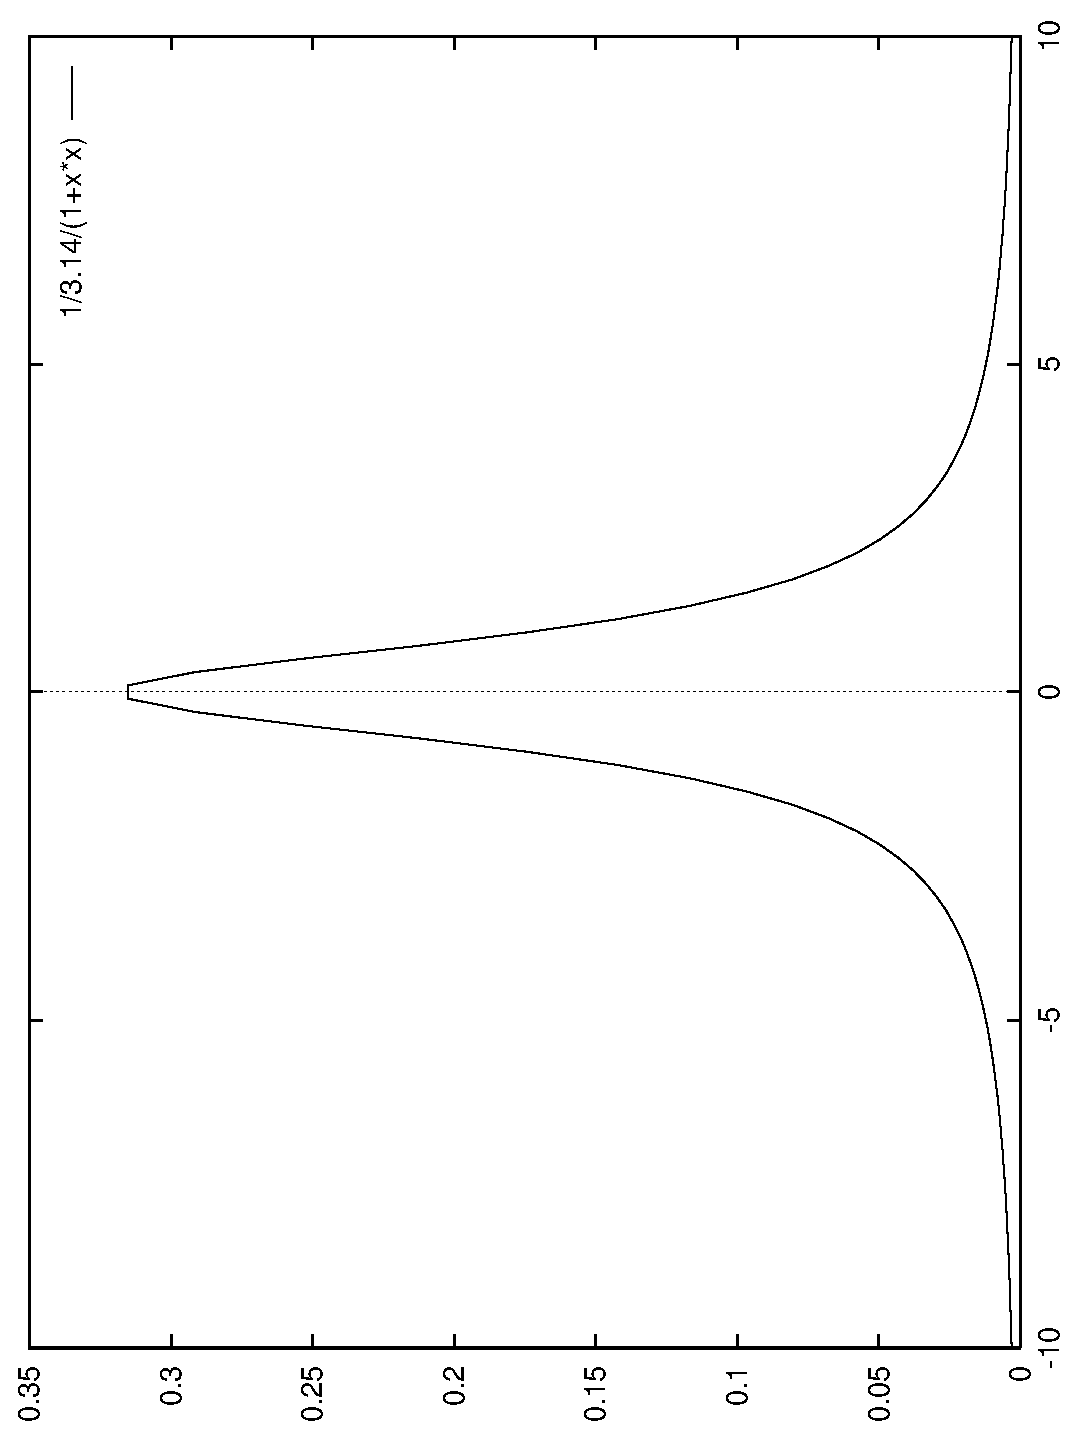
\includegraphics[height=12cm]{cauchy.eps}}\\
\caption{The Cauchy distribution.}
\label{Cauchy}
\end{figure}
\end{center}

\clearpage

\section{Public Methods}

\noindent
These methods can be used by all \cpp - programs, that have included the
header file Cauchy.h and the library EA.

\subsection{Constructors}

%---------------------------------------------------------------------------%
% 001
\index{Cauchy!( )} 
\setNormalInstance
\printEmptyMethodReturn
{}
{Cauchy}
{The default constructor. Generates the random generator of Cauchy distribution.}
{None.}
%---------------------------------------------------------------------------%

%---------------------------------------------------------------------------%
% 002
\index{Cauchy!( RNG\& rng )}
\setNormalInstance
\printMethodWithOneParam
{}
{Cauchy}
{RNG\&}
{rng}
{RNG class.}
{The constructor. Generates the random generator of Cauchy distribution.}
{None.}
{None.}
%---------------------------------------------------------------------------%

\vspace*{10mm}

\subsection{Operators}

%---------------------------------------------------------------------------%
% 003
\index{operator( )!( )} 
\setNormalInstance
\printEmptyMethodReturnSpecial
{double}
{operator( )}
{Gets the result of Cauchy distribution.}
{The factor which was occured by Cauchy distribution.}
{None.}
%---------------------------------------------------------------------------%

\clearpage

\subsection{The probability}

%---------------------------------------------------------------------------%
% 004
\index{p!( const double\& x )} 
\setConstInstance
\printMethodWithOneParam
{double}
{p}
{const double\&}
{x}
{The factor which you want to calculate the probability.}
{Returns the probability of {\em x}.}
{The probability.}
{None.}
%---------------------------------------------------------------------------%






